% AAAI-27 补充材料。
\documentclass[letterpaper]{article}
\usepackage[submission]{aaai2027}
\usepackage[hyphens]{url}
\usepackage{graphicx}
\urlstyle{rm}
\def\UrlFont{\rm}
\usepackage{natbib}
\usepackage{caption}
\frenchspacing

\usepackage{amsmath}
\usepackage{amssymb}
\usepackage{array}
\usepackage{booktabs}
\usepackage{listings}
\usepackage{tabularx}

\DeclareCaptionStyle{ruled}{labelfont=normalfont,labelsep=colon,strut=off}
\lstset{
  basicstyle=\footnotesize\ttfamily,
  numbers=none,
  aboveskip=4pt,
  belowskip=4pt,
  breaklines=true,
  columns=fullflexible,
  keepspaces=true,
  showstringspaces=false,
  tabsize=2
}

\newcolumntype{Y}{>{\raggedright\arraybackslash}X}

\setcounter{secnumdepth}{2}
\renewcommand{\thesection}{S\arabic{section}}
\renewcommand{\thesubsection}{\thesection.\arabic{subsection}}
\renewcommand{\thesubsubsection}{\thesubsection.\arabic{subsubsection}}
\renewcommand{\thetable}{S\arabic{table}}
\renewcommand{\thefigure}{S\arabic{figure}}
\renewcommand{\theequation}{S\arabic{equation}}

\pdfinfo{
/TemplateVersion (2027.1)
}

\title{Supplementary Material for SGDAgent: Hierarchical Spatio-Temporal Scene Graph-Driven Agent for Structured Long-Form Video Understanding}
\author{Anonymous Submission}
\affiliations{}

\begin{document}

% 待修改项总览（仅源码可见，不会进入 PDF）：
% 1. 核对实体对齐中类型不匹配和空描述的具体计分方式。
% 2. 在主稿中统一 FI 时间窗定义和 count/color 问题的直接路由条件。
% 3. 投稿前重绘 A1、A3，两张旧图目前仍包含与正文冲突的可见信息。

\maketitle

\noindent
This supplement complements the main paper with implementation details that
are useful for reproduction but too fine-grained for the main text.  It also
re-expresses the matched LVBench ablation as paired arithmetic differences and
revisits two archived case traces together with one text-only failure.  These
materials introduce no additional experiments.  They clarify how the reported
frame-level index is constructed and how individual trajectories should be
interpreted.


\section{Additional Reproducibility Details}
\label{sec:supp-reproducibility}

\subsection{Construction Settings}

The main paper specifies the model roles, graph hierarchy, and matched
evaluation protocol.  This section therefore focuses on the additional offline
settings needed to reproduce the frame-level index.
Table~\ref{tab:supp-settings} summarizes the extraction and sampling settings
retained from the implementation record.

\begin{center}
  \centering
  \small
  \setlength{\tabcolsep}{4pt}
  \begin{tabularx}{\columnwidth}{@{}lY@{}}
    \toprule
    \textbf{Component} & \textbf{Setting} \\
    \midrule
    Frame-graph extraction &
    \texttt{gpt-4.1}, temperature 0, at most 800 output tokens \\
    Frame sampling &
    candidates sampled every 5 seconds from 2 FPS decoded frames; when more
    than 120 candidates are available, 120 are uniformly retained over the
    full video \\
    \bottomrule
  \end{tabularx}
  \captionof{table}{Additional frame-level construction settings.}
  \label{tab:supp-settings}
\end{center}

\subsection{Frame-Graph Extraction and Normalization}

For each sampled keyframe, the extractor produces a compact set of typed
entities and directed relation triples.  The following core instruction
specifies the output contract.  It should not be read as the complete model
input: the preceding-frame graphs and video-level entity-registry context are
provided as described in the main paper.

\begin{lstlisting}
System:
You produce strict JSON only.

User:
Extract a compact frame-level scene graph from this image.
Return strict JSON with schema:
{"entities":[{"local_id":"e1","name":"person","type":"person",
"attributes":["standing"],"desc_text":"short description",
"confidence":0.0}],
"relations":[{"s":"e1","p":"holding","o":"e2","confidence":0.0}]}.
Rules: keep 1-8 salient entities, 0-12 relations, relation
predicate in snake_case.
\end{lstlisting}

The raw response is normalized deterministically before registry matching.
Post-processing lower-cases entity names and relation predicates.  Entity
types are restricted to \texttt{person}, \texttt{object}, \texttt{scene},
\texttt{animal}, \texttt{vehicle}, \texttt{food}, \texttt{text},
\texttt{location}, \texttt{building}, \texttt{clothing},
\texttt{instrument}, and \texttt{plant}.  Out-of-vocabulary types map to
\texttt{object}.  Meta-level terms such as \texttt{video}, \texttt{camera},
\texttt{subtitle}, and \texttt{background} are removed.  Relation predicates
outside the spatial, interaction, and state/action whitelist are discarded,
and confidence values are clipped to $[0,1]$.

\subsection{Cross-Frame Entity Alignment}

% 待确认：现有文档只定义了类型完全匹配时 R_type=1，没有说明类型
% 不匹配时的取值，也没有说明任一 description 为空时 R_desc 如何计算。
% 需要核对当前实现后再补充定义，不能根据旧附录自行推断。
Normalized frame graphs are processed sequentially into the video-level
entity registry.  For each new frame entity $e$, greedy online matching scores
the existing registry entities $\tilde e$ using
\begin{equation}
  \begin{split}
  R_{\mathrm{align}}(e,\tilde e)
  ={}&0.7R_{\mathrm{name}}(e,\tilde e)
  +0.2R_{\mathrm{desc}}(e,\tilde e)\\
  &+0.1R_{\mathrm{type}}(e,\tilde e),
  \end{split}
  \label{eq:supp-alignment}
\end{equation}
where the name and description terms are \texttt{SequenceMatcher} ratios, and
$R_{\mathrm{type}}$ is one for an exact type match.  The highest-scoring
candidate is merged when its score is at least $0.78$.  If no candidate reaches
the threshold, the frame entity is registered as a new entry.  A merge updates
the last-seen time, retains the larger confidence value, appends previously
unseen aliases, and unions the attribute sets.

\subsection{Frame-Inspection Instruction}

% 待修改（主稿 FI 定义）：主稿目前把 FI 的输入限定为 graph-proposed
% window，但 A1 的首次 FI 直接使用问题中给出的时间点。建议把主稿定义
% 改为 query-specified or graph-proposed window。补充材料当前使用中性的
% supplied time range，无需再改。
Graph retrieval proposes candidate regions, whereas frame inspection checks
raw visual evidence inside a supplied time range.  For each call, the
implementation uniformly samples at most 50 frames over that range and applies
the following instruction.

\begin{lstlisting}
System:
You are a helpful assistant to answer questions.

User:
Carefully watch the video frames. Pay attention to the cause and
sequence of events, the detail and movement of objects and the
action and pose of persons.
Based on your observations, answer the question using the visual
evidence. If no relevant content is found within the given time
range, return: `Error: Cannot find corresponding result in the
given time range.`.
Question: <question>
\end{lstlisting}

The instruction asks the verifier to return a fixed error string when the
supplied range contains no relevant evidence.  In the cases below, graph
results provide localization context, while $FI$ produces the visual attribute
or count judgment.  As the failure cases illustrate, that judgment is not
guaranteed to be correct.

\section{Verified Incremental Analysis}
\label{sec:supp-analysis}

The main paper reports absolute metrics for each matched LVBench
configuration.  Table~\ref{tab:supp-deltas} instead subtracts the source row
from the target row for selected comparisons.  C denotes the caption index.
F, S, and G denote the frame-level, segment-level, and global event graphs.
R, CG, and T denote query-type routing, confidence gating, and terminal
convergence.  The first three rows are nested index contrasts.  The remaining
rows compare control variants on the same C+F+S+G index, where ``No ctl.''
denotes that index with R, CG, and T disabled.  A negative call-count
difference means that the target configuration uses fewer calls.  This
arithmetic uses the one-decimal values displayed in the main-paper table,
rather than unrounded estimates reconstructed from raw counts, and introduces
no additional experiments.

\begin{center}
  \centering
  \small
  \setlength{\tabcolsep}{2.5pt}
  \begin{tabular}{@{}lrrrrr@{}}
    \toprule
    \textbf{Change} &
    \textbf{$\Delta$E2E} &
    \textbf{$\Delta$Ans.} &
    \textbf{$\Delta$Rate} &
    \textbf{$\Delta$LLM} &
    \textbf{$\Delta$FI} \\
    \midrule
    C $\rightarrow$ C+F                 & +4.4 & +3.3 & +2.3 & +1.2 & +1.3 \\
    C+F $\rightarrow$ C+F+S             & +3.6 & +3.0 & +1.4 & +4.7 & +2.7 \\
    C+F+S $\rightarrow$ C+F+S+G          & +1.6 & +0.2 & +2.0 & $-6.7$ & $-3.7$ \\
    \midrule
    No ctl. $\rightarrow$ R              & +5.1 & +2.9 & +3.4 & +0.1 & $-0.1$ \\
    R $\rightarrow$ R+CG                & +1.2 & $-0.5$ & +2.2 & +0.5 & +0.1 \\
    R $\rightarrow$ R+T                 & +1.3 & $-1.0$ & +3.0 & +0.1 & $-0.1$ \\
    R $\rightarrow$ R+CG+T              & +3.5 & $-0.9$ & +5.8 & +0.4 & $-0.3$ \\
    \bottomrule
  \end{tabular}
  \captionof{table}{Arithmetic differences derived from the main-paper
  component ablation.  Accuracy and answer-rate differences are percentage
  points; call-count differences are per question.}
  \label{tab:supp-deltas}
\end{center}

\paragraph{Index hierarchy.}
The first two contrasts pair positive end-to-end accuracy differences with
higher LLM and frame-inspection call counts.  The G contrast instead pairs
positive end-to-end accuracy and answer-rate differences with fewer calls.
These statements summarize the matched configurations and should not be read
as results from a separate retrieval experiment.

\paragraph{Agent control.}
Relative to R, the R+CG and R+T rows show answer-rate differences of $+2.2$
and $+3.0$ points, together with answered-accuracy differences of $-0.5$ and
$-1.0$ points.  These are conditional paired differences rather than additive
component effects.  In particular, the joint R$\rightarrow$R+CG+T contrast
should not be reconstructed by summing the separate R$\rightarrow$R+CG and
R$\rightarrow$R+T rows.

\section{Archived Case Studies and Limitations}
\label{sec:supp-cases}

The paired differences above summarize aggregate configuration behavior but
do not expose the mechanics of individual trajectories.
Figures~\ref{fig:supp-count-recovery} and~\ref{fig:supp-count-failure} provide
qualitative context through two archived case illustrations.  They are not
used to attribute the differences in Table~\ref{tab:supp-deltas}, and the
discussion below is restricted to evidence recorded in the corresponding
traces.

% 待修改（主稿路由条件）：
% - 主稿目前写成 count/color 问题直接进入 FI。
% - A1 的问题自带时间点，可以直接 FI；A3 和 Vancouver 的存档轨迹则先检索定位。
% - 建议明确：已有可用时间窗时直接 FI，否则可先用 GR/SR 定位检查窗口。
% - 条件写清前，A3 和 Vancouver 只能表述为存档定性轨迹，不能代表默认路由。

\paragraph{Graph-guided recovery after an incorrect count.}
The first case asks how many white lights were on at 45:08.  An initial $FI$
call returns the incorrect count of 34.  $GR$ and $SR$ then retrieve relevant
stage and lighting context before a targeted $FI$ call over the queried
instant returns the correct count of 24.  The graph evidence does not count
individual bulbs.  Its role in this trace is to provide stage and lighting
context before the visual evidence is inspected again.

% 待修改（A1 重绘，投稿前必须完成）：
% - 当前是旧版光栅图，不能原样提交，需要重新绘制并导出匿名矢量或高质量 PDF。
% - 工具名统一为 Global Event Graph Retrieval (GR)、
%   Segment-Level Graph Retrieval (SR) 和 Frame Inspection (FI)。
% - 层级名统一为 Global Event Graph、Segment-Level Graph、
%   Frame-Level Graph 和 Shared Entity Registry，并把 contain 改成 contains。
% - 明确首次 FI 使用问题给出的时间点，后续 FI 是图检索之后的重新检查。
% - 补回两次返回 30 的中间 FI，或继续将图片和 caption 明确标成 abridged。
% - 把 10+4+10 从 graph panel 移到最终 FI panel，计数必须归于原始视觉证据。
% - 删除内部 entity/frame ID 和重复的 light registry；如需保留，必须逐项核验。
% - 删除或修正过时的 seg_0184 候选时间，并核对全部事件、segment、frame 和时间戳。
% - 所有可见文字至少 9 pt，灰度下仍可读，不能只依赖颜色表达正误或层级。
% - 不要把带作者 metadata 的可编辑源文件放入匿名投稿包。
% - 图中应注明这是存档定性轨迹，不代表最终 R+CG+T 控制器的完整执行过程。
\begin{figure*}[t]
  \centering
  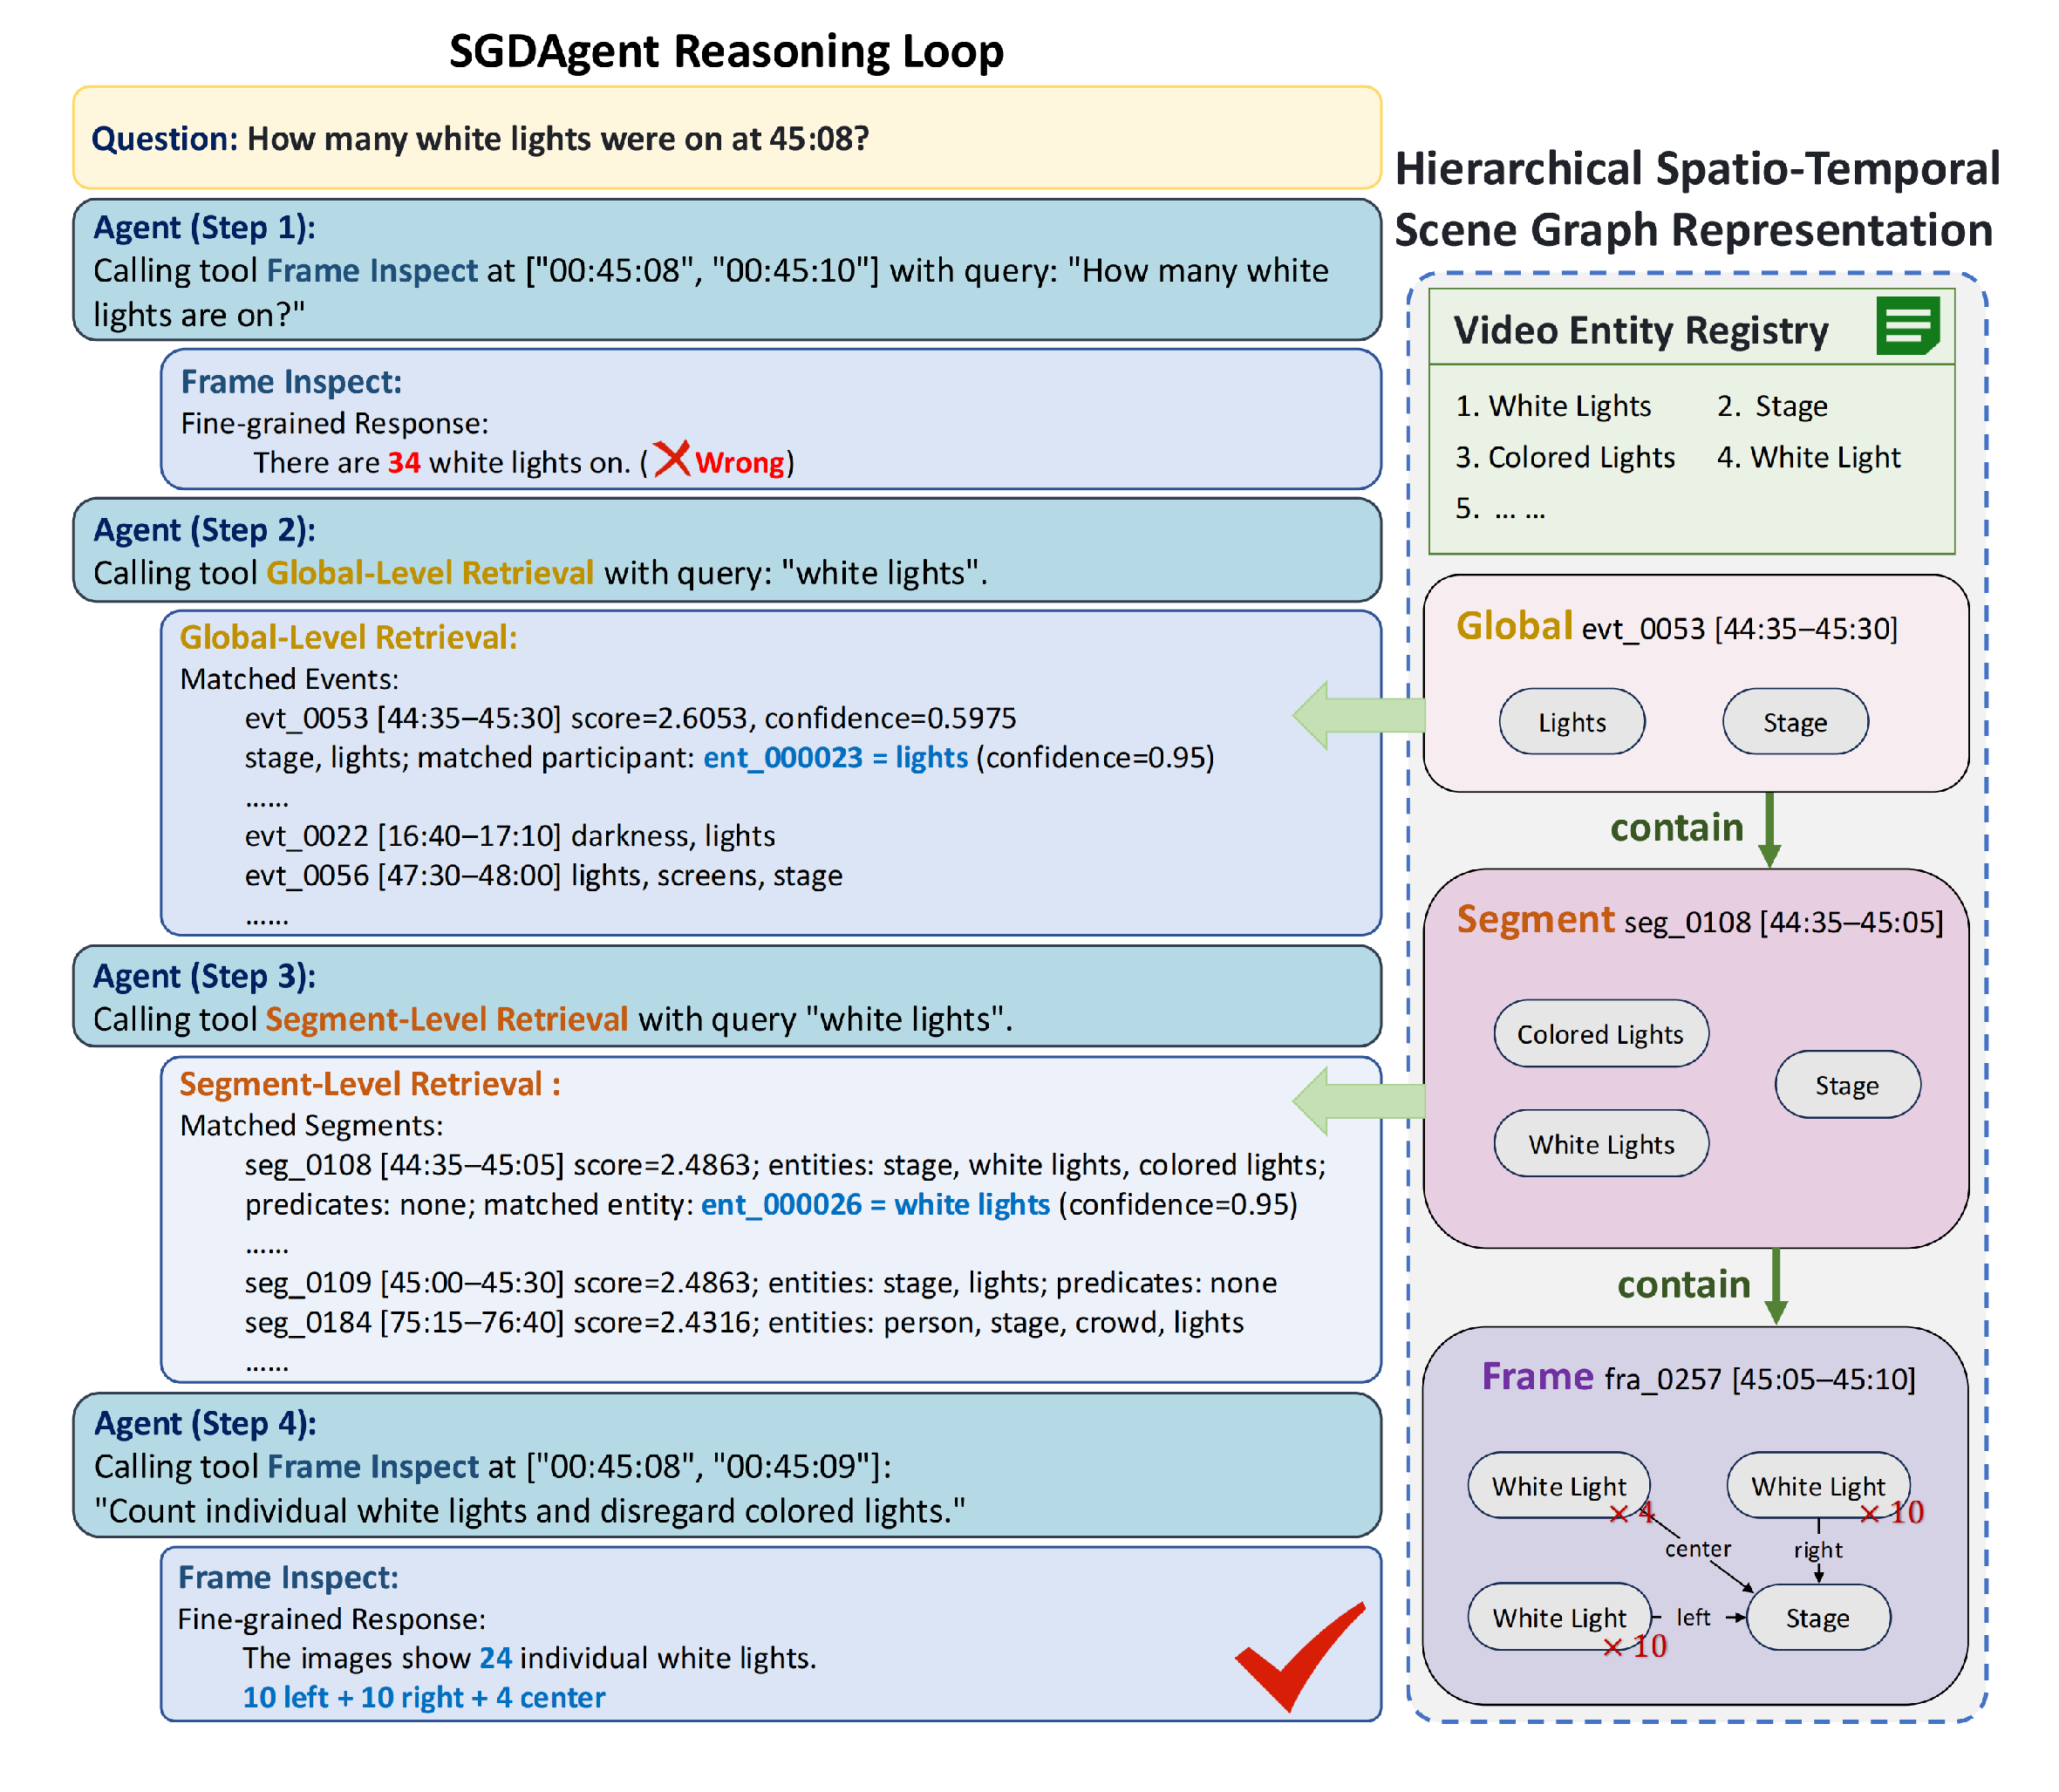
\includegraphics[width=\textwidth]{../paper/figures/Case_a1.pdf}
  \caption{Abridged archived LVBench success case (qid: \texttt{2256}).  The
  trajectory moves from an incorrect local count through graph retrieval to
  targeted visual reinspection.  The final value of 24 is obtained by $FI$.}
  \label{fig:supp-count-recovery}
\end{figure*}

\paragraph{Correct localization but incorrect numerical state.}
For the Taiyaki-capacity question, $GR$ retrieves the relevant cooking event,
and $SR$ surfaces the mold, Taiyaki, and Taiyaki maker in the corresponding
segment.  The hierarchy therefore reaches the correct cooking process, but
the retrieved graph evidence does not explicitly encode mold-slot occupancy.
The final $FI$ call separately overcounts the visible shapes and returns six
instead of the ground-truth four.  The trace records two distinct limitations:
missing numerical-state evidence and a visual counting error.

% 待修改（A3 重绘，投稿前必须完成）：
% - 当前是旧版光栅图，不能原样提交，需要重新绘制并导出匿名矢量或高质量 PDF。
% - 顶层 evt_* 节点应从 Segment 改成 Global Event。
% - 工具名统一为 GR、SR、FI，层级名使用当前正式术语，所有 contain 改成 contains。
% - 同时标出正确答案 (C) 4 和错误预测 (D) 6。
% - 分开呈现两个问题：检索图缺少 mold-slot-occupancy 关系，以及最终 FI 独立误计数。
% - 不要把错误答案完全归因于图表示缺失。
% - 标明这是存档定性轨迹，不能暗示 GR->SR->FI 是所有 count 问题的默认路线。
% - 删除冗余 score、confidence、长 query 和 entity list；内部 ID 仅在必要且核验后保留。
% - 所有可见文字至少 9 pt，灰度下仍可读，不能只依赖红绿颜色。
% - 不要把带作者 metadata 的可编辑源文件放入匿名投稿包。
\begin{figure*}[t]
  \centering
  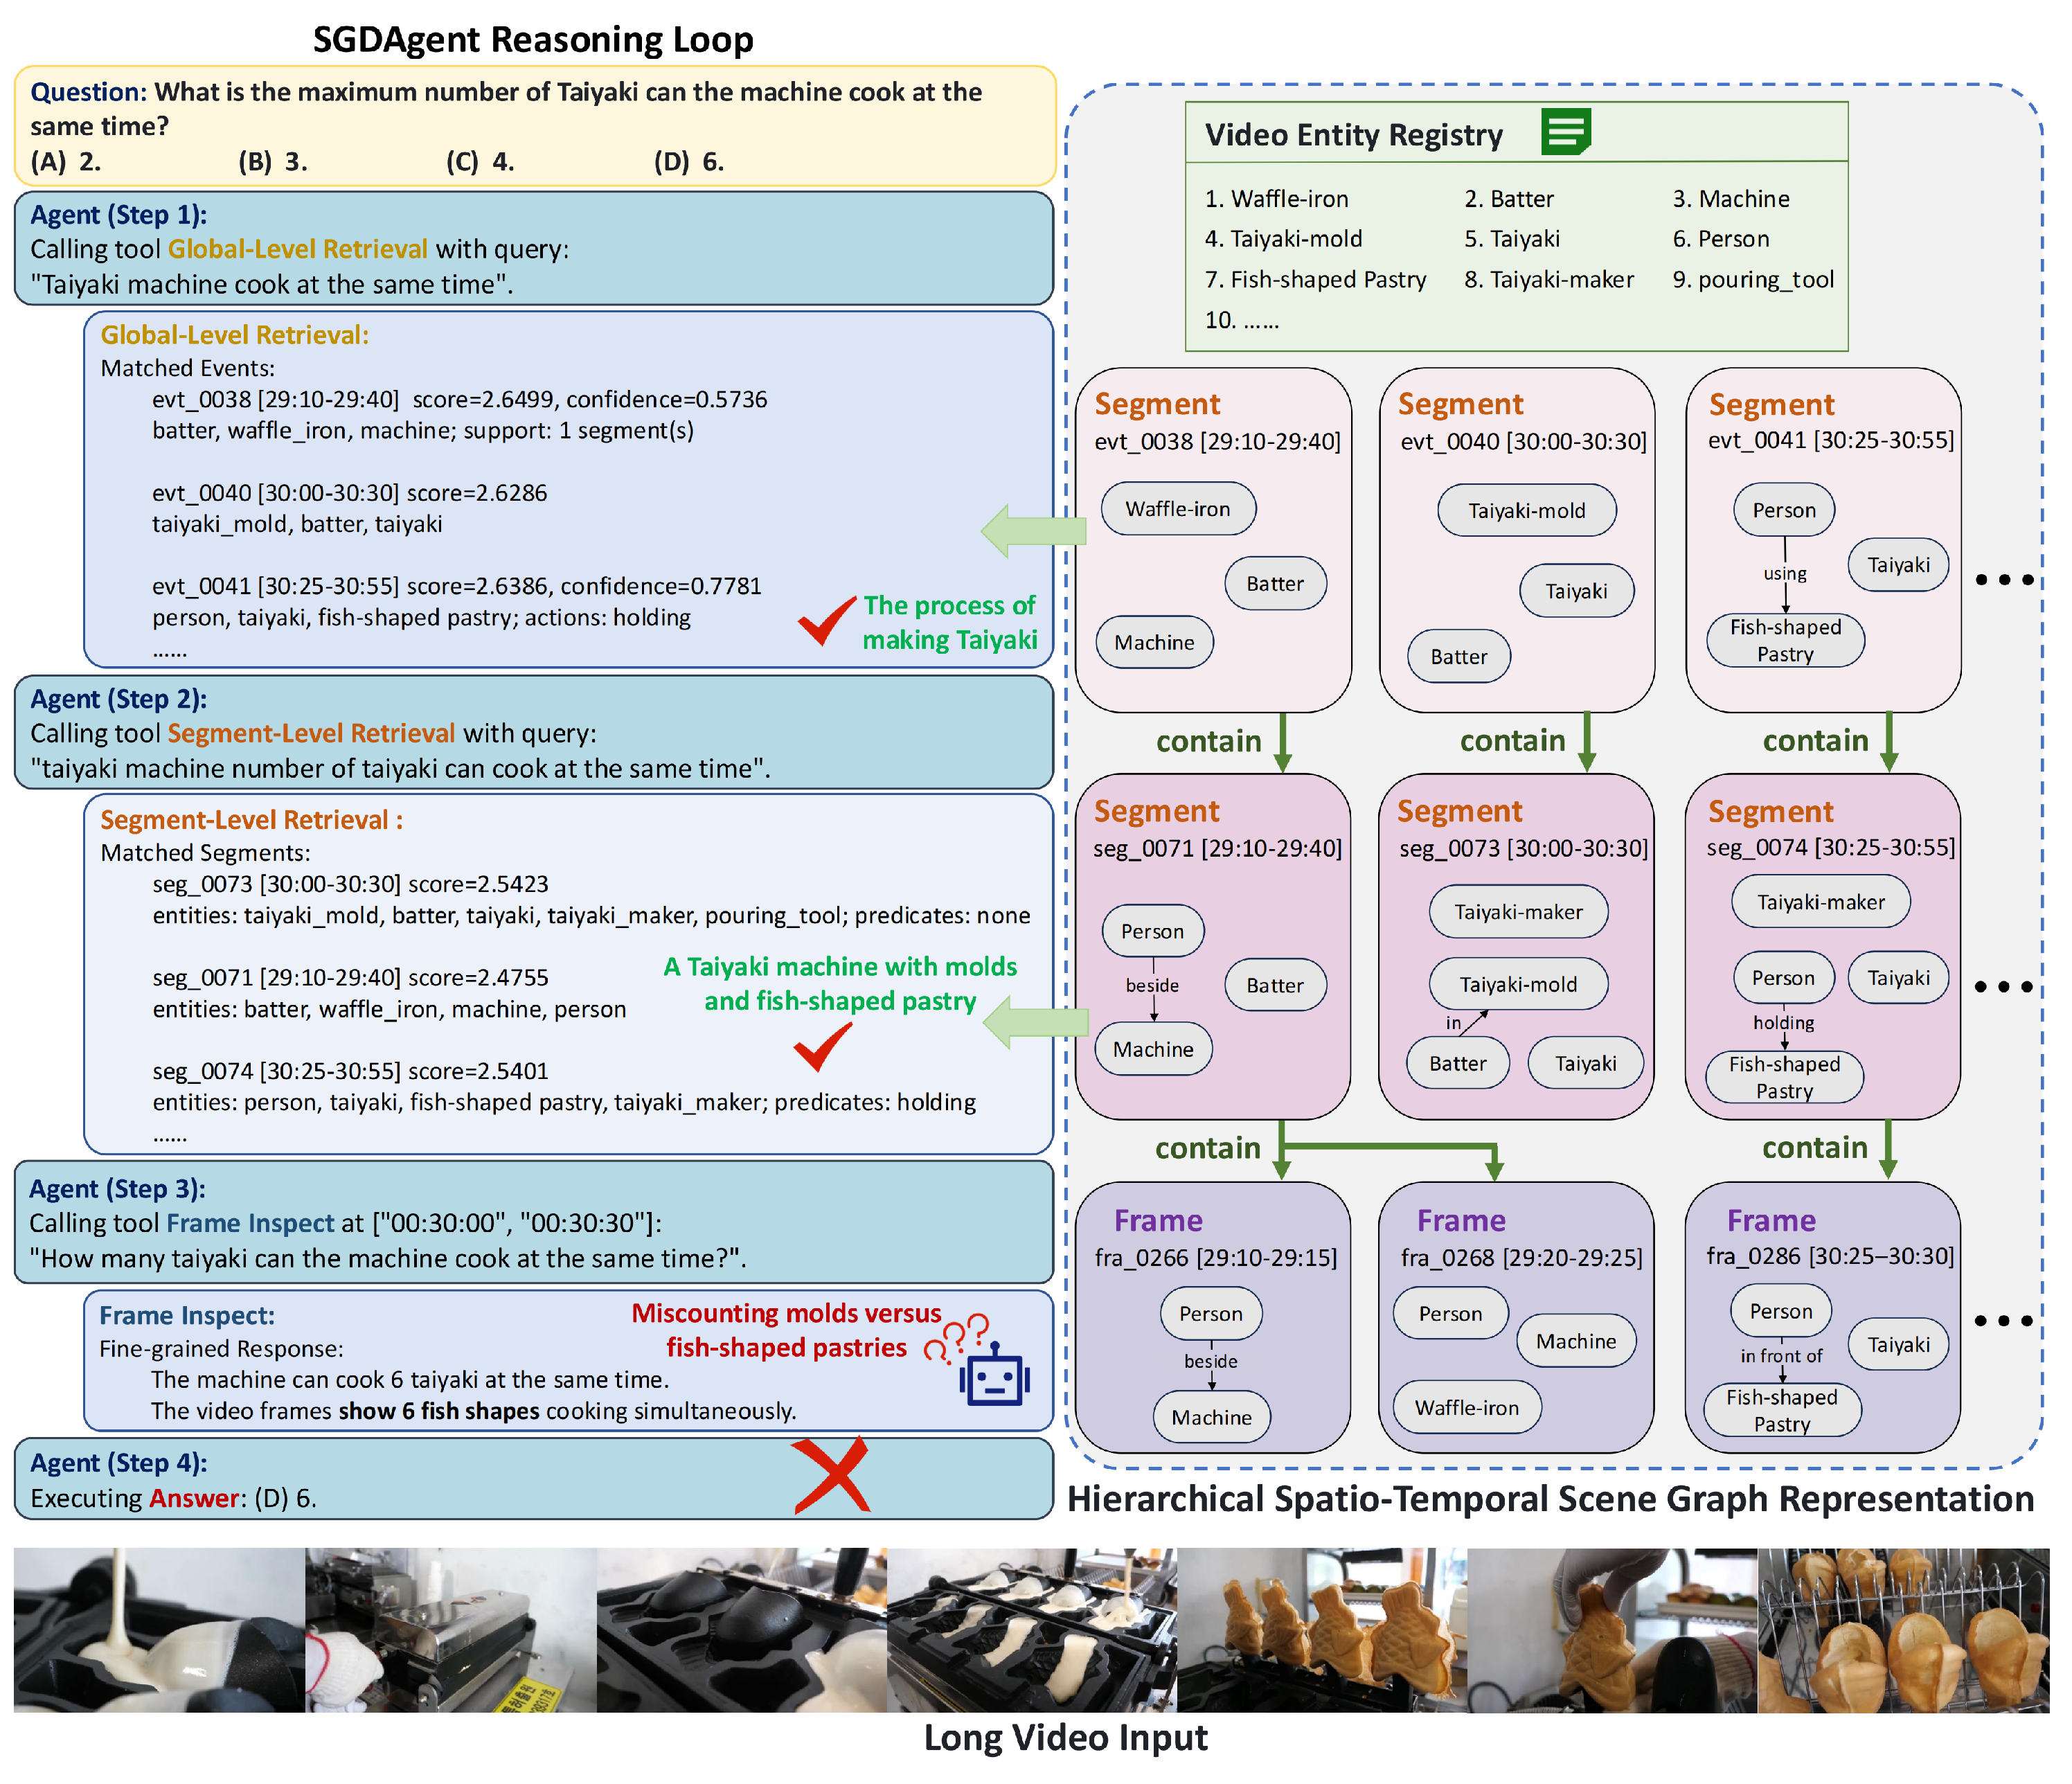
\includegraphics[width=\textwidth]{../paper/figures/Case_a3.pdf}
  \caption{Archived qualitative LVBench failure case (qid: \texttt{3322}).
  $GR$ and $SR$ locate the Taiyaki cooking process, but the retrieved evidence
  contains no explicit mold-slot-occupancy relation, and $FI$ returns six
  rather than the ground-truth four.}
  \label{fig:supp-count-failure}
\end{figure*}

\paragraph{Transient attributes and remaining limitations.}
The earlier appendix also reports a failure on the opening-light color of a
Vancouver gala performance.  $GR$ retrieves the broader performance, but the
event evidence contains no relation that isolates the exact opening instant.
The subsequent $FI$ call examines an interval that is too coarse to isolate
that instant.  It observes the dominant white illumination of the broader
performance and misses the brief opening state.  This failure differs from the
Taiyaki case: the Vancouver trace exposes a temporal-granularity limitation,
whereas the Taiyaki trace exposes missing count/state representation together
with a visual counting error.  These observations motivate finer temporal
slicing and explicit count/state relations.

\end{document}
